\documentclass{beamer}
\usepackage{tikz}
\usepackage{graphicx}
\usetikzlibrary{arrows,matrix,positioning}
\usetheme[progressbar=frametitle,sectionpage=none]{m}
\setbeamertemplate{bibliography item}[text]

\title{Dynamic Searchable Symmetric Encryption}
\author{Arpan Kapoor}
\institute{National Institute of Technology, Calicut}
\date{October 20, 2015}

\begin{document}

\maketitle

\begin{frame}
	\frametitle{Outline}
	\setbeamertemplate{section in toc}[sections numbered]
	\tableofcontents
\end{frame}

\section{Introduction}
\begin{frame}{Introduction}
\begin{itemize}
\item SSE allows client to encrypt data such that it can still be searched.
\item Application: Cloud storage.
\end{itemize}
\end{frame}

\section{Definitions}
\begin{frame}{Definitions}

\begin{block}{Symmetric Key Encryption}
\begin{itemize}
\item Same key for encryption and decryption.
\begin{columns}
	\column{0.33\textwidth}
	\[c = E_K(m)\]
	\column{0.33\textwidth}
	\[m = D_K(c)\]
	\column{0.10\textwidth}
\end{columns}
\end{itemize}
\end{block}

\begin{block}{Homomorphic Encryption}
\begin{itemize}
\item Permit computations on encrypted data.
\item Obtaining \(E_K(f(x))\) from \(E(x)\).
\end{itemize}
\end{block}

\end{frame}

\begin{frame}{Definitions}
\begin{block}{Psuedorandom Function}
\begin{itemize}
\item Polynomial time function whose output is indistinguishable from a
random function.
\[F \colon \{0,1\}^n \times \{0,1\}^s \rightarrow \{0,1\}^m\]
\item Given \(F\), \(K\), \(x_1, \dotsc, x_a\) and
	\(F_K(x_1),\dotsc,F_K(x_a)\), \\ \(F_K(x_{a+1})\) can't be predicted for any \(x_{a+1}\).
\end{itemize}
\end{block}
\end{frame}


\section{The SSE-1 scheme}
\begin{frame}{SSE-1 scheme}
\end{frame}

\section{Making SSE-1 dynamic}
\begin{frame}{Making SSE-1 scheme}
\end{frame}

\section{Example}
\begin{frame}[fragile]
\frametitle{Example}

\begin{center}
\begin{columns}
\column{0.05\textwidth}
\column{0.4\textwidth}
\footnotesize{\textbf{Index}}\\
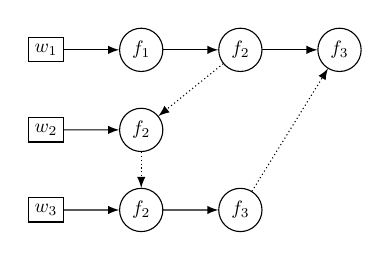
\begin{tikzpicture}[
roundnode/.style={circle, draw},
squarednode/.style={rectangle, draw},
every node/.append style={transform shape},
scale=0.7]
% Nodes
\node[squarednode] (w1) {\(w_1\)};
\node[squarednode] (w2) [below=of w1] {\(w_2\)};
\node[squarednode] (w3) [below=of w2] {\(w_3\)};
\node[roundnode] (f11) [right=of w1] {\(f_1\)};
\node[roundnode] (f12) [right=of f11] {\(f_2\)};
\node[roundnode] (f13) [right=of f12] {\(f_3\)};
\node[roundnode] (f22) [right=of w2] {\(f_2\)};
\node[roundnode] (f32) [right=of w3] {\(f_2\)};
\node[roundnode] (f33) [right=of f32] {\(f_3\)};
% Lines
\draw[arrows={-latex}] (w1) -- (f11);
\draw[arrows={-latex}] (f11) -- (f12);
\draw[arrows={-latex}] (f12) -- (f13);
\draw[arrows={-latex}] (w2) -- (f22);
\draw[arrows={-latex}] (w3) -- (f32);
\draw[arrows={-latex}] (f32) -- (f33);
\draw[densely dotted,arrows={-latex}] (f12) -- (f22);
\draw[densely dotted,arrows={-latex}] (f22) -- (f32);
\draw[densely dotted,arrows={-latex}] (f33) -- (f13);
\end{tikzpicture}
\column{0.3\textwidth}
\footnotesize{\textbf{Search Table} \(\mathtt{T}_s\)}
\(F_{K_1}(w_1) \rightarrow 4\)\\
\(F_{K_1}(w_2) \rightarrow 0\)\\
\(F_{K_1}(w_3) \rightarrow 5\)\\
\(\textsf{free} \rightarrow 6\)
\column{0.3\textwidth}
\footnotesize{\textbf{Deletion Table} \(\mathtt{T}_d\)}
\(F_{K_1}(f_1) \rightarrow 1\)\\
\(F_{K_1}(f_2) \rightarrow 5\)\\
\(F_{K_1}(f_3) \rightarrow 4\)
\end{columns}

\vspace{2ex}
\hrule
\includegraphics[trim=55mm 175mm 43mm 60mm, clip, width=0.9\textwidth]{../paper/pg_0005.pdf}
\end{center}
\end{frame}

\section{Conclusion}

\plain{Questions?}

\begin{frame}[allowframebreaks]
	\frametitle{References}
	\nocite{*}
	\bibliographystyle{abbrv}
	\bibliography{main}
\end{frame}

\end{document}
